
\section{Computational Models}

While this thesis only used Serpent 2 \cite{leppanenjaakko_serpent_2015} for modeling, work to improve HTGR modeling in one program can inform efforts in another.  Therefore, this chapter includes discussion of software beyond Serpent 2.

\subsection{Serpent 2}

In order to create and model complex geometries, Serpent 2 uses constructive solid geometry (CSG), which defines homogeneous material cells using user-defined universes, cells, lattices, and specially-defined nested objects to define particle and pebble geometries.  Using these special objects, and the particle dispersal routine in Serpent 2, we can create TRISO particles and pebble bed reactors.  Previous work has tested with up to 60 million individual particles \cite{noauthor_serpent_nodate}.

Physics use a combination of classical kinematics, ENDF reaction laws, and random sampling.  For particle transport, Serpent 2 uses surface tracking and Woodcock-delta tracking.  For material data, it uses ACE format libraries for microscopic cross sections, and pre-generates macroscopic cross sections before beginning transport.  To further speed-up calculations, Serpent 2 uses a unionized energy grid.  Serpent 2 validation studies compare against MCNP, and validation is ongoing for radiation shielding and criticality safety analysis \cite{noauthor_serpent_nodate}.  While the differences between Serpent 2 and other Monte Carlo programs are usually marginal, Serpent 2 experiences the same issues validating its results as other Monte Carlo programs (related to small differences in data libraries \cite{noauthor_serpent_nodate}).

\subsection{Work in Other Software}

A 1996 effort to improve MCNP developed a new sampling method for Monte Carlo.  Its creators dubbed the version of MCNP that used the sampling algorithm as MCNP-BALL.  After testing by performing isotopic inventory and criticality calculations the MCNP-BALL code results were accurate to 0.2\%.  The work developing MCNP-BALL also answered a weakness in core simulation due related to difficulties in modeling reactors with a so-called "double-heterogeneity" - having two or more types of pebble in a single reactor \cite{murata_new_1997}.

An additional look into MCNP HTGR simulations examined the ability to create what would normally be a stochastic geometry with a uniform design.  Specifically, it used a body-centered-tetragonal (BCT) and hexagonal close pack (HCP) lattice for the TRISO particles.  For low packing fractions, such as ones seen in TRISO-in-pebble packing, the particles are far enough apart that the differences between two crystal lattice structures are insignificant.  In smaller cores, with adequate reflectors, the differences between the pebble packing lattices were more significant, but manageable.  Additionally, the effect of completely homogenizing the coating of the TRISO particles - blending them with the graphite matrix - lowered $k_{eff}$.  For methods using less dramatic homogenization methods, such as blending the four TRISO coatings into one uniform layer, the computational load decreased, and the results were marginally different from the 4-coating TRISO particle \cite{karriem_mcnp_2001}.

BEAU, or Burnup Equilibrium Analysis Utility \cite{cisneros_pebble_2013}, models depletion and multiple burnup states for a continuously refueled pebble bed reactor. It uses the multiple burnup state method (MBSM) to do so, which improves on most full-core pebble bed computational methods by including all burnup states for a pebble rather than homogenizing them into a representative average pebble.

BEAU is a Python-based coupling software that combines either MCNP5 or Serpent with ORIGEN2, using new interface inspired by the MOCUP software named mocup.py.  Mocup.py takes the output files from an MCNP5 or Serpent simulation, and turns them into an object for aiding in depletion simulations.  BEAU is for fuel cycle analysis and finding the maximum burnup equilibrium.  It was bench-marked against results for a pebble-bed HTGR in INL's PEBBED and VSOP \cite{cisneros_pebble_2013}.

\subsection{Fuel Modeling}

BEAU aided in the design of a pebble bed fluoride high temperature reactor (PB-FHR) named the Mark-1 PB-FHR \cite{cisneros_pebble_2013}.  The Mark-1 PB-FHR handles pebble locations using a face-centered cubic (FCC) lattice in which all burnup states seen in the reactor are present.  Assuming a uniformly mixed core, the closeness of the different burnup compositions in the lattice provide a fairly good estimation of the true core.

A more general study examined the effects of pebble packing on the core neutronics in an HTGR \cite{turkmen_effect_2012}.  Rather than model a full core, the study created a unit cell as a reference.  The study considers body centered cubic (BCC) and hexagonal close-packed (HCP) lattice unit cells.  Instead of using a variety of compositions to represent an equilibrium, middle-of-life (MOL) core, the study used an enrichment of 9.6\%  - lower than the standard \~15\% for fresh HTGR pebble-fuel - for all pebbles.  For each lattice configuration, tests varied the fuel/moderator (F/M) ratio, and examined the effects on core neutronics and isotopic compositions.  The analysis shows no significant difference between BCC and HCP cells.  The study determined it would be difficult to select a truly 'optimal' energy spectrum vis-\`{a}-vis minimizing the accumulation of particularly harmful fission products.  The author concluded that F/M ratios less than 1/1 favor reducing actinide inventories, while ratios greater than 1/1 can reduce the generation of fission products that would corrode the layers of the TRISO fuel.

Earlier work on HTGRs by General Atomic determined the composition of discharged thorium/uranium prismatic fuel elements.  The study assumed fuel recycling to complement the proposed breed/burn fuel cycle.  Additionally, the fuel cycle assumes the reactor can start with an initial feed material of 93\% U-235, which is currently infeasible (at least in commercial reactors in the United States) \cite{hamilton_htgr_1976}.


\section{Modern HTGRs}

The following discusses more recent  HTGR designs, which are the inspiration for Sangamon200 and Sangamon20.

\subsection{PBMR}

The PBMR is a South African pebble bed HTGR design.  While it did not ultimately make it to construction, its design has offered invaluable insight to later HTGR pebble bed designs.  The PBMR is heavily based on the German High Temperature Reactor (HTR) design, and has a nameplate thermal power of 400 MW, with inlet-outlet temperatures of 500 \textdegree C to 900 \textdegree C.  It is a modular design, with each unit containing a graphite moderated, helium-cooled-core housed in a steel pressure vessel.  In accident scenarios, the PBMR would rely on passive safety features using conduction and convection to provide cooling.

\begin{figure}[h!]
\centering
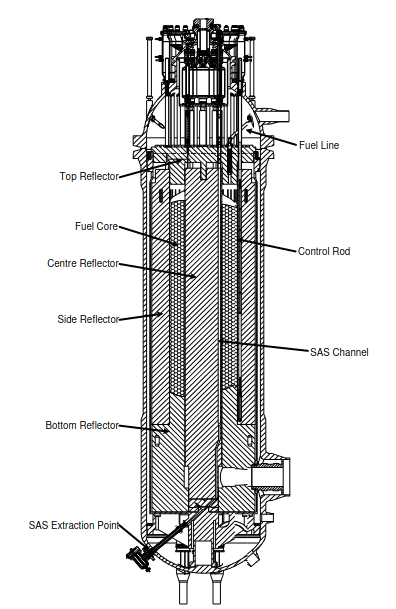
\includegraphics[width=0.5\linewidth]{figures/pbmr-v-cross-sect}
\caption{PBMR Schematic: Vertical Cross-section \cite{venter_pbmr_2005}}
\label{fig:pbmr-v-sect}
\end{figure}

Each core unit would hold around half a million pebbles, which used LEU based TRISO particles as the fuel form.  These TRISO particles are pressed into a 2.5 $\left[cm\right]$ radius graphite sphere, which then has an additional 0.5 $\left[cm\right]$ thick layer of graphite pressed around it, to form a 3.0 $\left[cm\right]$ radius pebble - around the size of a billiard ball.  The pebbles would undergo a six-pass cycle to reach a target end burnup of 92,000 $\left[\frac{MWd}{tU}\right]$ \cite{venter_pbmr_2005}.

As part of the design process, multiple 400 MWth PBMR benchmarks underwent development and testing.  An early benchmark using MCNP5 simplified the fuel by assuming an equilibrium pebble enrichment of 9.6 wt\%, a common tactic.  It also uses a BCC lattice for pebble positions.  Its calculated $k_{eff}$ differed from previous MCNP4b results by as much as 1,315 pcm \cite{kim_monte_nodate}.

An improved benchmark modeled the original VSOP benchmark more closely.  A full-core model used a cubic array to map TRISO particles inside the pebbles, while an HCP lattice defines pebble locations \cite{albornoz_mcnp_nodate}.  As an improvement on previous benchmarks, it adds back in the fuel regions from the VSOP model, which tracks pebbles in channels and axial layers to simulate their movement through the core.  However, it does simplify these layers, see Figure \ref{fig:fuel-regions}, below:

\begin{figure}[H]
\centering
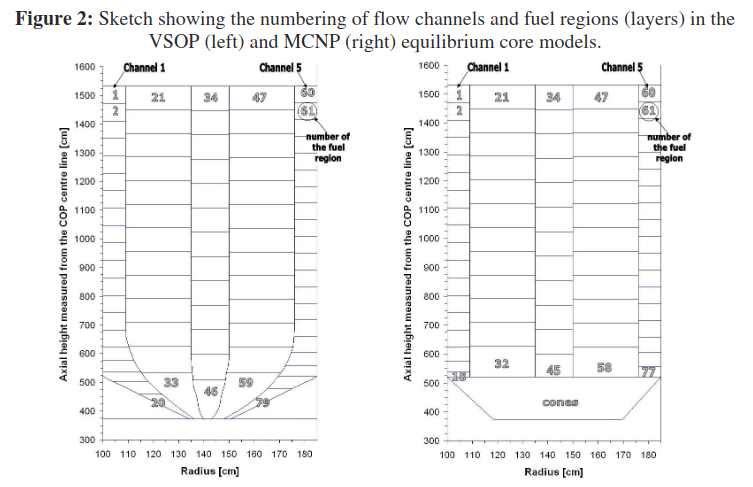
\includegraphics[width = 0.9\textwidth]{figures/bench-fuel-regions.png}
\caption[Diagram of fuel regions in an equilibrium PBMR core model]{Diagram of fuel regions in an equilibrium PBMR core model, reproduced from \cite{albornoz_mcnp_2006}.  Axial fuel zones defined for use in MCNP model validation (right) against a previous VSOP model (left).}
\label{fig:fuel-regions}
\end{figure}

To simplify, the different pebble burnups in each region are averaged.  This study also investigated the effects of different pebble packing arrangements, but rather than use a full-core, a representative one-meter cube of pebbles defines a reference model.  The study tested random, HCP, BCC, and FCC at packing fractions of 0.542 and 0.61.  It found that across identical packing fractions, differences in reactivity were small, though $k_{eff}$ values differed by several standard deviations \cite{albornoz_mcnp_nodate}.

An additional work performed criticality and burnup calculations using MCNP5 and MONTEBURNS 2.0.  It, like many other pebble-bed models, uses an averaged 9.6\% enriched fuel to simulate an equilibrium core \cite{noauthor_criticality_2011}.  It tested three pebble arrangements:  a BCC lattice with a packing fraction of 0.68, a random arrangement with a packing fraction of 0.61, and a simple cubic (SC) lattice with a packing fraction of 0.52.  The initial $k_{eff}$ were similar: 1.2395, 1.2357, and 1.2223, respectively.  However, the effective full power days (EFPDs) and end of life burnup required to reach an end $k_{eff}$  of 1.02 differed considerably.  BCC required 1200 EFPDs and ended on 99,000 $\frac{MWD}{T}$, random ended on 1000 EFPDs and a burnup of 92,000 $\frac{MWD}{T}$, and the SC lattice required 800 EFPDs and achieved a final burnup of 86,000 $\frac{MWD}{T}$ \cite{noauthor_criticality_2011}.  However, for the random pebble arrangement, which was used to validate the model, the disagreement in excess reactivity was approximately 14\%.

A study using VSOP focused on possible power peaking and the formation of hot spots.  To test hot spots forming, a mass of fresh pebbles were purposefully introduced in the fuel region corresponding to the peak power.  Even for a very large cluster of fresh pebbles, maximum fuel power only increased by 16\%.  However, the volumetric power density increased to 18.66 from 11.32 $\frac{MW}{m^3}$ \cite{reitsma_investigation_2005}.  Of note, this scenario is highly unlikely - the region of highest power is three meters into the core, by which point fresh pebbles would have been burned slightly.  This is in addition to the already accidental loading of over one thousand fresh pebbles at once.

\subsection{Next Generation Nuclear Plant (NGNP)}

Like the PBMR, the NGNP did not make it to construction.  However, work in analyzing reactor designs and materials still applies to other work.  The NGNP project downselected its design choices to two reactors - a prismatic HTGR and a pebble-bed HTGR.  While the NGNP project eventually opted for the Areva prismatic HTGR design \cite{noauthor_areva_nodate} due to reasons related to pebble costs, studies noted that, technologically speaking, there was no inherent advantage or disadvantage bewteen the two technologies \cite{inl_basis_2011}.

Even though the reactor didn't make it to construction or operation, a plethora of research conducted in support of the NGNP project is applicable to similar reactors.  One such study is a whole-core depletion study of the the proposed prismatic HTGR design.  It uses a once through fuel cycle, and assumed an average burnup of 100-150 $\left[\frac{GWd}{t}\right]$ after an 18 to 24 month stint in the core.  Much of the work from this study is applicable only to prismatic designs, namely the effects of the number of batches cycling, and fuel shuffling on core neutronics \cite{tkkim_whole-core_nodate}.

\subsection{X-energy}

Based on experience from the PBMR project, the X-energy Xe-100 is a 200 MWt HTGR pebble-bed SMR.  It is similar in design to all of its predecessors, featuring LEU TRISO particle fuel in 3.0 $\left[cm\right]$ radius pebbles.  While the Xe-100, or similar design, is not in operation as of this publication, the project is still ongoing.  It is this reactor, and by extension the PBMR, that the micro-reactor described in this thesis is most heavily influenced by.

The Xe-100 uses approximately 220,000 pebbles in a six-pass cycle, and fuel pebbles identical to the ones intended for the PBMR \cite{harlan_x-energy_2018}.  However, while the number of passes is unchanged, the target end burnup for the pebbles is higher, at 160,000 $\left[\frac{MWd}{tU}\right]+$ \cite{agnihotri_intrinsically_2017}.  Another key difference from the PBMR beyond size is the lack of central reflector.

While the Xe-100 is not built, there have been studies conducted by ORNL providing data on the production and material properties of the PBMR-type fuel pebble.

\subsection{HTR-10}

The HTR-10 is a 10 MW, HTGR model.  Multiple studies exist examining the effects of pebble and TRISO arrangement on the HTR model.  These studies primarily work with the Reactor Monte Carlo (RMC) or MCNP5 programs.  A base benchmark study created the HTR-10 in MCNP.  Pebbles contained 8335 TRISO particles on average, dispersed in a cubic lattice.  Pebbles, meanwhile, are in a BCC arrangement, such that F/M ratios and void fractions stay constant \cite{kim_monte_2005}.

A later study used RMC to study the explicit modeling of the random nature of both the pebbles and particles in the core, a 'double heterogeneity' \cite{ she_explicit_nodate}.  The Random Sequential Addition (RSA) method was used to distribute the TRISO particles within the pebbles (the packing fraction was less than 30\%, the maximum RSA can achieve).  The Discrete Element Method (DEM) dispersed pebbles.  To simplify the model, it assumed that all pebbles have identical TRISO dispersal patterns.  Testing showed this caused little ($\sigma$ less than 0.00014) error between this simplification and a model using different TRISO arrangements in each pebble.  The RMC model had good agreement with VSOP HTR-10 simulations \cite{ she_explicit_nodate}.

Other work with the HTR-10 introduces a new method of explicit random particle dispersion for use in RMC, called the Random Universe Geometry method (RUG).  RUG improves on RSA by allowing a higher particle packing fraction, and on the DEM by being faster and simpler to implement \cite{liu_random_2018}.  Whenever a particle enters a cell that is stochastic, the algorithm randomly samples from a list of possible materials, and determines the contents of the cell mid-transport.  The RUG method has good agreement with preliminary testing using HTR-10 benchmarks \cite{liu_random_2018}.



